\chapter{Group Anomaly Detection (GAD) }  
 \label{sec:staticGAD}
%\section{ Group Anomaly Detection (GAD) Techniques} \label{Sec:GAD}
% Brief paragraph 
After setting up the group deviation detection  problem and describing the general framework for methods in previous sections, we now  explain specific GAD techniques in further detail. 
 GAD involves comparing multiple groups and identifying groups with significantly different statistical properties.  Following the problem definition in Section   \ref{Sec:Problem}, 
${\bf G}_m= \Big ( {X}_{mnv}\Big) \in \mathbb{A}^{N_m \times V}    $ 
where domain $\mathbb{A}$ depends on the   input data type such as  categories, discrete value or continuous variables.
 GAD methods are explained by descriptive key components from Section   \ref{Sec:Problem} in  categories of discriminative methods,  generative models and hypothesis tests. 

% A description of GAD techniques is provided 


\section{ Discriminative Methods } 
 In GAD, a discriminative method classifies input groups into regular and anomalous behaviours.     
We  elaborately discuss two state-of-the-art discriminative models for detecting group anomalies.  Firstly One-Class Support Measure Machine (OCSMM)   proposed by Muandet and Sch\"olkopf \cite{OCSMM} %supports unsupervised learning for classifying group behaviours,  OCSMM 
is an unsupervised method that maximises the margins between two classes using a separating hyperplane.  
 Another discriminative model Support Measure Data Description (SMDD)   proposed by Guevara et al. \cite{SMDD} is similar to OCSMM however uses a supervised approach  based on a minimising the  volume sets that contains the majority of groups in a training set.  % are contained in boundaries (soft or hard) of a volume set. 
  Both methods can handle continuous and discrete input data where it is assumed that the statistical properties of group deviations can be differentiated based on certain  optimisation criteria. 
  
 In this analysis, each  group   is associated with a probability measure where observations  are assumed to be  independent and identically distributed (iid). 
Formally, %on the  space $(\Omega,\mathcal{F})$
given an  outcome space $\Omega$ and $\sigma$-algebra $\mathcal{F}$, we define a set of probability measures $\mathcal{P}=\{\mathbb{P}_1,\dots,\mathbb{P}_M\}$  
where each function is given by $\mathbb{P}_m: \, \Omega \to [0,1]
$ for $m=1,\dots, M$. 
  % The set of all probability measures  $\mathcal{P}_\Omega$  is defined on the probability space $(\Omega,\mathcal{F},\mathbb{P})$. 
If groups  ${\bf G}_1,{\bf G}_2,\dots,{\bf G}_M$ exhibit regular behaviour then they have iid probability distributions specified by $\mathbb{P}_1,\dots,\mathbb{P}_M$.   
 In both OCSMM and SMDD, mean embedding functions are applied to transform groups into points in a reproducing kernel Hilbert space (RKHS). 
   Let $\mathcal{H}$ denote the RKHS of probability measures with   kernel $k:\Omega \times \Omega  \to\mathbb{R}$.  Group behaviours are characterised using mean kernel embedding functions as defined by 
 \begin{align}
\mu :  \mathcal{P}\to \mathcal{H}, \quad\mathbb{P}_m \mapsto \mu_{\mathbb{P}_m}=E_{\mathbb{P}_m} [ k({\bf G}_m,\cdot) ] =\int_{\Omega} k(u,\cdot)\, d\mathbb{P}_m(u).  \label{KMF}
 \end{align}
 for $m=1,\dots,M$. 
 

  

\subsection{ One-Class Support Measure Machine (OCSMM) }
 Muandet et al. \cite{OCSMM} propose OCSMM for  discriminating between regular and anomalous  group behaviours using a parametrised hyperplane. OCSMM maximises
 the margin between two classes as separated based on the hyperplane.  
{  Since OCSMM is  analogous to one class support vector machines  \cite{OCSVM}, we describe a linear hyperplane for vector ${\bf x}$ as } 
\[ %f_{\bf w}(x) = 
\big\langle {\bf w}, {\bf x} \big \rangle = \rho \]
where parameters $({\bf w}, \rho)$ are the weights and bias term for parametrising a separating hyperplane respectively.  Regular behaviours are further away from  the origin than anomalous instances. 

OCSMM allows the user to select the expected proportion of group anomalies in the training data as denoted by  $\nu \in (0,1)$.  Since group anomalies are assumed to occur much less frequently that regular groups,  OCSMM learns patterns from one-class that exhibits  the dominant behaviour in a dataset.  
For more flexible margins in a separating hyperplane, 
slack variables $\xi_1,\dots,\xi_M$ are  introduced such that the parameters  of a separating hyperplane are estimated by optimising the following problem %results in the optimisation problem 
%\vspace{-1cm}
 \begin{align}
&\min_{(  \rho, {\bf w},\boldsymbol \xi)} 
\frac{1}{2} \langle {\bf w},{\bf w} \rangle_{\small \mathcal{H}} - \rho +  \frac{1}{\nu M} \sum_{m=1}^M
\xi_m  \label{minW} \\
\mbox{with con}\mbox{straints: } &  \langle {\bf w} ,  \mu_{\mathbb{P}_m } \rangle_\mathcal{H} \ge \rho - \xi_m \mbox{ and } \xi_m \ge 0 \mbox{ for } m=1,\dots,M   \nonumber
\end{align}
%and the parameters ${\bf w},\,\rho$ and  $\boldsymbol\xi$ are
 The first term in Equation (\ref{minW}) represents  minimising the error or distance of separating data points from the origin. The slack variables offer a more flexible description of a separating hyperplane where penalty term $1/{\nu M}$ represents the trade-off between the distance of a hyperplane from the origin and the upper bound on expected number of group anomalies in a training set.  
Equation (\ref{minW}) can be solved by introducing Lagrange multipliers $\boldsymbol \alpha$ where the estimated hyperplane is %estimated by %with weights % $\bf w$ %simplified as 
\begin{align*}
 f_{\bf w}(\mu_{\mathbb{P}_m } ) = \big\langle {\bf w},\mu_{\mathbb{P}_m } \big \rangle_\mathcal{H} \quad %= \sum_{l} \alpha_l \, \langle \mu_{\mathbb{P}_m}, \mu_{\mathbb{P}_l}\rangle_\mathcal{H} \\
\mbox{ where }{\bf w}= \sum_{m=1}^M \alpha_m  \mu_{\mathbb{P}_m} \mbox{ and } \sum_{m=1}^M \alpha_m=1
%0 \le \alpha_m \le \lambda
\end{align*} 
 
The following schema describes OCSMM in four key components:   
 \begin{enumerate}[1.]
\item Characterisation function $f_1({\bf G}_{train})={\bf w}$: \\ The training set of group behaviours contains information about  $\mu_{\mathbb{P}_1},\dots, \mu_{\mathbb{P}_M}$.  In particular, the weight function of a separating hyperplane characterises a group training set by
\[{\bf w}= \sum_{m=1}^M \alpha_m  \mu_{\mathbb{P}_m}\] 
 \end{enumerate}
 %
 \begin{enumerate}[2.]
 \item Characterisation function $f_2({\bf G}_{test})=\mu_{\mathbb{P}_m}$: \\ 
The $m$th group is characterised by the mean embedding function $\mu_{\mathbb{P}_m}$.  Intuitively group observations are mapped onto the RKHS as group feature  representations. 
\end{enumerate}
 %
\begin{enumerate}[3.]
\item Measure $ \mathcal{D}\big( f_1({\bf G}_{train}), f_2({\bf G}_{test})\big )$ using a separating hyperplane: \\
The separating hyperplane compares characterisation functions ${\bf w}$ and $\mu_{\mathbb{P}_m }  $ with
$ \big\langle {\bf w},\mu_{\mathbb{P}_m } \big \rangle_\mathcal{H}%\sum_{l} \alpha_l \, \langle \mu_{\mathbb{P}_m}, \mu_{\mathbb{P}_l}\rangle_\mathcal{H}
$.   
 For a deeper understanding of this measure, consider  
\begin{align*}
 \big\langle {\bf w},\mu_{\mathbb{P}_m } \big \rangle_\mathcal{H}= \sum_{l} \alpha_l \, \langle \mu_{\mathbb{P}_m}, \mu_{\mathbb{P}_l}\rangle_\mathcal{H} 
\end{align*} 
where the kernel similarity on probability measures based on empirical samples is 
%To ensure the kernel similarity estimated on empirical samples   %K(\hat{\mathbb{P}}_m,\hat{\mathbb{P}}_l)=
\begin{align}
\langle \hat{\mu}_{\mathbb{P}_m},\hat{\mu}_{\mathbb{P}_l} \rangle_\mathcal{H}  
=
\frac{1}{N_m   N_l } \sum_{i=1}^{N_m}
 \sum_{i'=1}^{N_l} k\Big( X_{mi} , 
 X_{li'}  \Big)  \label{kernelest}
 \end{align}
%and $X_{mi}$ is the $i$th observation in the $m$th vector. 
%The following assumptions are imposed 
A reasonable approximation using empirical estimates for probability measures, requires   $||  \mu_{\mathbb{P}_m}  - \hat{\mu}_{ \mathbb{P}_m}  || $ is bounded   for $m=1,\dots,M$.   

  The selection of kernel similarity function $k$ is important in the detection of group anomalies.
When $k$ is chosen as a characteristic kernel such as a  Gaussian   kernel, the representative function $\mu$ is injective, that is there is a distinct mapping of groups onto the RKHS. The anomalous measure and classification threshold in  OCSMM are also dependent on the selection of kernel function. Table \ref{Tab:Kernel} provides examples where given a particular choice of reproducing kernel  $k$ in Equation (\ref{kernelest}), OCSMM characterises different statistical properties of  groups. 

 % of kernel functions that captures different statistical properties of groups. %For instance, a linear kernel only captures the behaviour of the first moment of a distribution while the  Gaussian RBF describes infinite moments.\\[2mm]

\end{enumerate}

 \begin{table}[H]
 
\begin{center}
\tabcolsep=0.25cm
 \scalebox{0.9}{
\begin{tabular}{p{15mm}ccp{20mm} } 
 \hline\\[-2mm]
Type & Reproducing Kernel $k(u,v)$  & Kernel Similarity $K(\mathbb{P}_m,\mathbb{P}_{l}  )$ & Moments  \\[1mm]
\hline \\[-4mm]
 \hline\\[-2mm]
Linear & $\langle  u,v \rangle $  & $0\, [Av \mbox{ if } \mathbb{P}=N(A,1)] $ & First\\[2mm]
Quadratic & $\langle  u,v \rangle ^2$   &  $v^2$ & Second \\[2mm]
Quadratic &  $(\langle  u,v \rangle +1)^2$ & $v^2+1$ & First \& Second \\[2mm]
Gaussian RBF & $\displaystyle \exp \bigg( {-\frac{||u-v||^2}{2\sigma^2} } \bigg)$ & $ \displaystyle \frac{1}{\sqrt{2}}\exp \bigg({-\frac{||v||^2}{4} } \bigg)  $ & Infinite
\\[-2mm]
& & $(\sigma^2=1)$ & 
 \\[1mm] \hline
\end{tabular}
}
\end{center}
%\vspace{-1cm}
 \caption{ Examples of different kernels for probability distribution $\mathbb{P}=N(0,1)$. % and the Gaussian RBF has a bandwidth or tuning parameter  $\sigma>0$.  
 }
 \label{Tab:Kernel}
\end{table}

 \begin{enumerate}[4.]
\item  Threshold $\epsilon= \rho$: \\  The  threshold term for OCSMM represents a bias parameter for the separating  hyperplane. This threshold is calculated from   groups with probability measures that are mapped closest to the separating hyperplane. In fact,   support measures provide a description for the separating hyperplane such that the $m'$th group with $ 0 <\alpha_{m'} < \displaystyle \frac{1}{\nu M}$ is a support measure  that satisfies 
\[ \rho  %=f_{\bf w}(\mu_{\mathbb{P}_m } )
 = \big\langle {\bf w},\mu_{\mathbb{P}_{m'} } \big \rangle_\mathcal{H}= \sum_{l} \alpha_l \, \langle \mu_{\mathbb{P}_{m'} }, \mu_{\mathbb{P}_l}\rangle_\mathcal{H}  \]
Then a threshold for anomalous groups is     \[\hat{\rho}=  \sum_{l} \hat{\alpha}_l \, \langle \hat{\mu}_{\mathbb{P}_{m'}}, \hat{\mu}_{\mathbb{P}_l}\rangle_\mathcal{H} \] 
A group anomaly is classified by a parametrised hyperplane if
$   \big\langle \hat{\bf w},\hat{\mu}_{\mathbb{P}_m } \big \rangle_\mathcal{H}  < \hat{\rho}$. Thus group deviations are closer to the origin than regular group behaviours. 
 \end{enumerate}
 
  
\subsection{ Support Measure Data Description (SMDD) } 
 Guevara et al. \cite{SMDD} propose SMDD for  distinguishing between regular and anomalous  group behaviours by learning the dominant behaviour (one-class)   using minimum volume (MV) sets. {  Since SMDD is  analogous to support  vector data description \cite{SVDD}, we introduce a common MV-set for a vector ${\bf x}$ where an enclosing hypersphere with center $\bf c$ and radius $R$ is described by } 
 %The discriminative functions for SMDD is based on fitting on minimum volume set on  training data.      \[|| \hat{\mu}_{\mathbb{P}_m} -  \hat{\bf c} ||^2 \]
%describes an minimum volume sphere
\[ ||{\bf x}  -{\bf c}||^2 \le R^2 \]
 Since anomalous groups may be present in a training set, a penalty term is introduced. The penalty parameter $\lambda >0$ represents the trade-off between the volume of a  hypersphere and 
 the expected proportion of anomalous groups in a training set. 
 For a more flexible radius boundary, slack variables $\big\{\xi_m \big\}_{m=1}^M \ge 0$ are also introduced where SMDD %a MV-set %$\bf c$ and $R$
 involves minimising the objective function 
 \begin{align}
 &\min_{(R,{\bf c}, \boldsymbol\xi) }   R^2+\lambda \sum_{m=1}^M \xi_m \label{SMM1}  \\
\mbox{with constraints: } &||\mu_{\mathbb{P}_m}  -{\bf c}||^2 _\mathcal{H}\le R^2  +\xi_m  \mbox{ and } \xi_m  \ge 0 \mbox{ for } m=1,\dots,M  \nonumber
\end{align}
 The first term in Equation (\ref{SMM1}) accounts for radius of a volume set while the second term accounts for less strict radius boundary for a MV set. 
 
 Similar to OCSMM, we describe the key components of SMDD as follows.
 \begin{enumerate}[1.]
\item Characterisation function $f_1({\bf G}_{train})= {\bf c}$: \\
 By combining kernel embedding functions  $\mu_{\mathbb{P}_1},\dots, \mu_{\mathbb{P}_M}$, the center of an enclosing hypersphere is estimated by  
\[{\bf c}= \sum_{m=1}^M \alpha_m  \mu_{\mathbb{P}_m}\] 
The value $\bf c$ characterises  group information on the training set with weights that are optimised in a different way to OCSMM. A special case occurs when a spherical normalisation of mean embedding functions is applied with   
\[  \langle \mu_{\mathbb{P}_m}, \mu_{\mathbb{P}_l}\rangle_\mathcal{H} \mapsto  \frac{ \langle \mu_{\mathbb{P}_m}, \mu_{\mathbb{P}_l}\rangle_\mathcal{H}} { \sqrt{\langle \mu_{\mathbb{P}_m}, \mu_{\mathbb{P}_m}\rangle_\mathcal{H}  \langle \mu_{\mathbb{P}_l}, \mu_{\mathbb{P}_l}\rangle_\mathcal{H}}} \]
From Guevara et al. \cite{SMDD},  SMDD and OCSMM are equivalent under a spherical transformation  that preserves the injectivity  of the Hilbert space mapping.
 \end{enumerate}
%
 \begin{enumerate}[2.]
\item Characterisation function $f_2({\bf G}_{test})=\mu_{\mathbb{P}_m}$: \\ 
Similar to OCSMM, the $m$th group is characterised by  mean embedding function $\mu_{\mathbb{P}_m}$. However even though the group characterisation in SMDD is identical to OSCMM, the weights are optimised based on different criteria. \end{enumerate}
 %
\begin{enumerate}[3.]
\item Measure $ \mathcal{D}\big( f_1({\bf G}_{train}), f_2({\bf G}_{test})\big )$: \\
The anomalous score for the $m$th group is calculated by \[ || \hat{\mu}_{\mathbb{P}_m} -  \hat{\bf c} ||^2_\mathcal{H}  \]
where it is assumed that  $||  \mu_{\mathbb{P}_m}  - \hat{\mu}_{ {\mathbb{P}}_m } || $ is bounded  for   groups $m=1,\dots,M$. 
\end{enumerate}
%
\begin{enumerate}[4.]
\item Threshold $\epsilon={R}^2$: \\ In SMDD, the estimated radius 
$\hat{R}^2$   of an enclosing sphere provides a threshold for group deviations.  Suppose that the $m'$th group has a support measure with $ 0 <\alpha_{m'} < \displaystyle \lambda$ then the radius threshold is estimated as
\[ \hat{R}^2  =  || \hat{\mu}_{\mathbb{P}_ {m'} } -  \hat{\bf c} ||_\mathcal{H}^2  \]
\end{enumerate}
A group anomaly is detected if it is not enclosed by a MV set, that is 
$ || \hat{\mu}_{\mathbb{P}_{m} } -  \hat{\bf c} ||^2_\mathcal{H} > \hat{R}^2$. Thus  group deviations occur  outside of the boundaries of an estimated minimum volume set. 

\section{Generative Models for Known Groups Memberships} \label{Sec:G}
Generative models for group anomaly detection   assume that data is generated from an underlying statistical process involving observed data variables $\bf X$,  latent variables $\mathcal{H}$ and model parameters $\Theta$.   Hidden or latent variables are introduced to capture the unseen interaction between observed  data variables. Generative methods in topic modelling applications infer  latent statistical properties representing topics in documents.  Usually structural values (such as the number of latent variables) are selected prior to model inference. % whereas model parameters  control the distribution for a data generating process.
A group anomaly is characterised by irregular proportions of inferred topic variables. %We will explain generative models for detecting anomalous groups in the application of topic modelling. 
For reference, Table \ref{Notation} introduces the topic modelling  terminology and notation that will be discussed  in this section. %for  generative models for detecting group anomalies. 

 \begin{table}[h]
\begin{center}
 	\renewcommand{\arraystretch}{0.98}
 	\tabcolsep=0.2cm 
 \scalebox{1}{
\begin{tabular}{ ccl%lp{45mm}p{45mm}p{45mm}
} 
 \hline\\[-2mm]%[-4mm]
%  \multicolumn{3}{l}{ {\bf Algorithm 1 } \, Generative Process of GMM}\\%[-3mm]%[-2mm]%& Assumptions & Strengths & Weakness   \\%[1mm]
Quantities & Symbol & Description \\[1mm]
 \hline \\[-3mm]
 Fixed&$M$ & Number of groups \\
  Values & $N_m$ & Number of words/documents in   $m$th group \\
%$\mathcal{S}$ 
  & $N$& Total number of words/documents   \\[2mm]
\hline \\[-3mm]
 Structural & $K$ & Number of topics \\
Values  &$J$& Types of regular group behaviours\\[2mm]
\hline \\[-3mm]
Observed  & $ X_{mn} $ & The $n$th word/documents in $m$th group \\
Variables  & $ X_{\cdot,n} $ & The $n$th word in entire corpus$^*$  \\
${\bf X}$& $ Y_{nn'} $ & The connection of the $n$th word with the $n'$th word  \\[2mm]
 %& $ {\bf G}_{m} $ & The $m$th group is a collection of random variables \\[1mm]
% & $\mathcal{C}_{n}$ &  The group indicator of the $n$th  word \\[1mm]
 \hline \\[-3mm]
 &$\theta$ & Parameter of topic distributions\\
     &$\phi$ &  Parameter of word distributions \\%  &$\chi$ 
  Model   &$\gamma$ & Parameter of genre distributions\\
%  \hline \\[-3mm]Variational  Parameters $\Delta$
Parameters   & $\alpha$ & Prior parameter on topic distributions\\
$\Theta$ &$\beta$ &  Prior parameter  on word distributions\\
 & $\eta $ & Prior on group membership distributions \\
 & $\bf B$ & Blockmodel matrix for  connection probabilities    \\[2mm]
 \hline\\[-3mm]
 &$ Z_{mn} $ & Topic  indicator for $n$th word in $m$th group \\
%&$ Z_{\cdot,n} $ & The topic associated with $n$th word in  entire corpus  \\
 Latent   & $ \chi_{m} $ & Genre  indicator for  $m$th group  \\
Variables & $ \theta_{m} $ & Topic probabilities for $m$th group (when priors are introduced)  \\
$\mathcal{H}$  & $ \phi_{m} $ & Word probabilities for $m$th group (when priors are introduced)  \\
& $\tilde{G}_n $ & Group indicator for the $n$th data instance \\
& $\pi_n $ & Group membership probability for the $n$th data instance \\[2mm]
\hline \\[-3mm]
%& $ C_{pq}$ & The link associated with $p$th and $q$th  word \\\hline \\[-3mm]
 \multicolumn{3}{l}{*Model inference is applied to  entire corpus without incorporating group information.} \\ 
\end{tabular}
}
\end{center}
 \caption{Notation for generative models  in the context of topic modelling. }
 \label{Notation}
\end{table} 

Generative models are explained in terms of four key components as follows: %introduced in   \ref{Sec:Problem}. 
\begin{enumerate}[1.]

\item Characterisation function $f_1({\bf G}_{train})= \boldsymbol\Theta$: \\   Generative models  infer a set of model parameters $\boldsymbol\Theta$   to characterise a group training set ${\bf G}_{train}=\{{\bf G}_{1},\dots,{\bf G}_{M}\}$. Structural values such as expected number of topics are selected based on the lowest value of Alkaike Information Criteria (AIC) \cite{AIC} 
 or Bayesian Information Criteria (BIC) \cite{BIC}. 
For observed data variables ${\bf X}$ and model parameters $\boldsymbol\Theta$, the
AIC and BIC scores are respectively calculated  by
\begin{align}%\centering
& \hspace{8mm} AIC({\bf X}, \boldsymbol\Theta)=-\ln L({\bf X}| \boldsymbol\Theta)+|
\boldsymbol\Theta | \label{AIC} \\[1mm]
& \hspace{25mm}\mbox{ and} \nonumber \\ 
& BIC({\bf X}, \boldsymbol\Theta)=-\ln L({\bf X}| \boldsymbol\Theta)+\frac{1}{2}|
\boldsymbol\Theta|\, \ln (|{\bf X}|)\label{BIC}
\end{align}
where $L({\bf X}|\boldsymbol\Theta)$ is the likelihood of observed data variables given the model parameters and $|\cdot|$ is the number of elements in a  vector or matrix. 
Gershman and  Blei \cite{NPB} further describe how automated parameter selection for generative models is achieved through Bayesian non-parametrics however this has a relatively greater computational  time and complexity. 
\end{enumerate}



 
 
\begin{enumerate}[2.]
\item Characterisation function $f_2({\bf G}_{test})=Z_m$: \\ 
For unsupervised approaches, a test set coincides with a training set. We consider the $m$th group as the test set with  ${\bf G}_{test}={\bf G}_{m}$.  Many topic models have been applied to GAD applications. Topic models assume a generative process of data and  infer latent statistical properties such as topic proportions in documents. A topic variable indicates that a word is associated with a particular topic.  The characterisation function of the $m$th group is the inferred topic variable $ Z_m$.  
To obtain topic variables, generative models firstly estimate the posterior distribution of observed data and latent variables under given model parameters with %$\mathcal{H}$,  %is estimated by 
\begin{align}
p({\bf X},\mathcal{H}| \boldsymbol\Theta) \label{pos}
\end{align}
There are many ways to infer latent variables in  generative models. %involving Dirchlet processes.  
Monte Carlo Markov Chain (MCMC) methods iteratively  sample from a probability distribution that theoretically converges to the posterior distribution in Equation (\ref{pos}) %. The equilibrium of a sampled distribution is difficult to assess and 
however has a slow computation especially for larger datasets. Gilks et al. \cite{MCMC} describe different MCMC algorithms for estimating distributions in practice. If applicable, collapsed Gibbs sampling offers a faster computational time for generative models as implemented by Porteous et al. \cite{fastCGS}.


 Another approach to infer model parameters   is by   computing an Expectation-Maximisation (EM) algorithm  
  using variational inference. In variational inference, $q(\mathcal{H}|\Delta)$ is a  distribution of latent variables  $\mathcal{H}$ with variational parameters $\Delta$. A variational distribution approximates the  posterior distribution in Equation (\ref{pos}). By  minimising Kullback-Leibler (KL) divergence between distributions, the optimal variational parameters are computed by 
\[ 
\Delta^* =  \underset {\Delta }{\mbox{argmin}} \;
D_{KL} \Big( p({\bf X},\mathcal{H}|   \boldsymbol\Theta) \,\Big|\Big|\,  q(\mathcal{H}|\Delta) \Big)
\]
where $D_{KL}$ is the KL divergence. For a faster and scalable procedure when dealing with large datasets, stochastic variational inference is proposed by Hoffman et al.    \cite{stochasticVI}    where the posterior distribution in  Equation (\ref{pos}) is approximated by iteratively  updating noisy gradient estimates of the objective function. 
\end{enumerate}
 %For $K$ topics and $T$ themes, this requires a search to minimise the AIC or BIC over $K$ and $T$. 
 
\begin{enumerate}[3.] 
\item Measure $ \mathcal{D}\big(f_1({\bf G}_{train}), f_2({\bf G}_{test})\big )$: \\
Generative models usually compute likelihood scores  from model parameters to determine which groups exhibit a higher degree of anomalous activity.  
 The anomalous behaviour of a test group ${\bf G}_{m}$ is  quantified by the negative log-likelihood score
 \begin{align}
 \mathcal{S} ({\bf G}_{m}) = - \ln P({\bf G}_{m} | \Theta) \label{GroupL}
 \end{align}
 The likelihood score in Equation (\ref{GroupL}) is heavily influenced by individual outliers and more effectively characterises point-based group anomalies. On the other hand, distribution-based group anomalies are more appropriately quantified by a likelihood score involving topic variables  
\begin{align}
 \mathcal{S} ({\bf G}_{m}|Z_{m}) = - E_{Z_{m}} [\ln P({Z}_{m} | \Theta) ] 
  \label{TopicL}
\end{align}
Since topic variables are latent,  group scores in Equation  (\ref{TopicL}) are estimated through Monte Carlo integration using Gibbs sampling.  
\end{enumerate}

 

\begin{enumerate}[4.]
\item Threshold $\epsilon $ is  selected by domain experts: \\  
Since generative methods only calculate likelihood scores that are relative to a particular dataset, it is difficult to obtain a universal threshold value.  Higher  scores are interpreted as groups with a greater degree of anomalous activities. A threshold is arbitrarily selected based on a proportion of  groups with the highest scores.  In most  generative models, group deviations are associated with  scores that are greater than a subjectively chosen  threshold. Alternatively, it is possible that additional analysis such as a  bootstrapping procedures  provide generative models with a  threshold estimate.  
\end{enumerate} 
 
We now discuss the details of GAD generative models when group memberships are known a priori. Groups of related instances are naturally defined in many applications. For example,  a document is a group of words whereas a corpus is a collection of documents.    
 In topic modelling applications, statistical properties of groups are described in terms of topic proportions. We now highlight similarities and differences between state-of-the-art generative models for detecting group anomalies.  

 { \it Gaussian Mixture Model (GMM)}: \\ 
The Gaussian Mixture Model (GMM) is a commonly used probabilistic generative model in applications from high energy particle physics \cite{GMM} to speaker verification \cite{speakerV}.   
Figure \ref{Fig:GMMvsLDA} (a) illustrates the generative process of GMM in plate representation. $N$ words in the corpus are assumed to be generated  from $K$ different topic-word distributions. 
Given $K$ topics, a topic variable for the $n$th word is generated from a Multinomial probability with parameter $\theta $ such that $Z_{\cdot,n} \sim \mbox{Multi}(\theta )$.    
The posterior distribution in Equation (\ref{pos}) is based on data variables ${\bf X}= \{ X_{{\cdot},n} \}_{n=1}^N $, latent variables $\mathcal{H}=\{Z_{\cdot,n}\}_{n=1}^N$ and model parameters $\Theta=\{\theta,\phi\}$.  Since GMMs do not incorporate  group information (document context),  model parameters are inferred  over the entire dataset so that GMM detects point-based group anomalies rather than distributed-based group deviations.  

\subsection{ Latent Dirichlet Allocation (LDA) }
 Latent Dirichlet Allocation (LDA) proposed by Blei et al. \cite{LDA} is a  popular and widely used generative model  for topic modelling. Figure \ref{Fig:GMMvsLDA} (b) depicts the generative process of LDA in plate representation. 
Given a particular document (group), a word is generated from one of $K$ topic-word distributions with $Z_{m} \sim \mbox{Multi}(\theta_m )$.  LDA  introduces 
  Dirichlet priors on Multinomial distributions with $\theta_m \sim \mbox{Dir}(\alpha)$  to account for  uncertainty of unknown topic quantities and also prevent  overfitting a large number of topics  to high-dimensional text data.

%The posterior distribution in Equation (\ref{pos}) is based on data variables ${\bf X}= \{ X_{mn} : n=1,\dots,N \mbox{ and } m=1,\dots,M \} $ and model parameters $\Theta=\{\alpha,\phi\}$. 
 The  posterior distribution in Equation (\ref{pos}) is estimated for observed documents   with 
 \begin{align*}
& \mbox{Observed Data:  \;\; \quad}  {\bf X}= \{{\bf G}_{1},{\bf G}_{2},\dots,{\bf G}_{M} \}\\
 & \mbox{Latent Variables: \quad}    \mathcal{H}=\{\theta_{m},Z_{m} \}_{m=1}^M  \\
 & \mbox{Model Parameters: \;\,}  \Theta=\{\alpha,\phi\} 
 \end{align*} 
   where ${\bf G}_{m} = \{ X_{mn} \}_{n=1}^{N_{m}}$ represents a group as a document of words.    
 
 
% Algorithm 1 and 2 respectively describe the  generative processes of GMM and LDA.
  A key difference in LDA compared to GMM is  the ability to incorporate a hierarchical structure due to document (group) information. This is illustrated in Figure \ref{Fig:GMMvsLDA} where observed variables are given by $X_{mn}$ in LDA which takes accounts for document context rather than fitting over all of the observed words $X_{\cdot,n}$ in GMM.  %The number of words within a document in LDA  can also be modelled by a Poisson distribution however we do not include this in our analysis.  
As there are many extensions of LDA, we focus on generative models that  specifically relate to  GAD. % \cite{ }discovers anomalous documents
The Dirichlet distribution in LDA reduces potential overfitting however since a Dirichlet prior is a uni-modal distribution,  a single optimal topic mixture is fitted for all documents. LDA detects point-based and  distributed-based group anomalies however  it cannot capture multiple types of regular group behaviours.



\begin{figure*}[!t]
    \centering
      \begin{subfigure}[H]{0.8\textwidth}
        \centering
        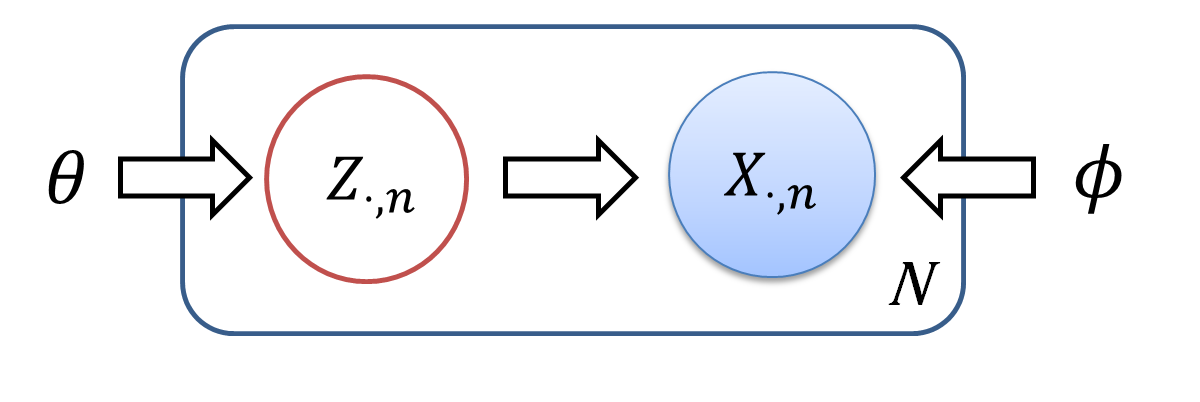
\includegraphics[width=0.75\linewidth, height=2.8cm,
        trim=0cm 0.2cm 1cm 0cm]{FIGURES/GMM}
        \caption{Plate representation for GMM }
    %\vspace{-8mm}
    \end{subfigure}
    \begin{subfigure}[H]{0.8\textwidth}
        \centering
        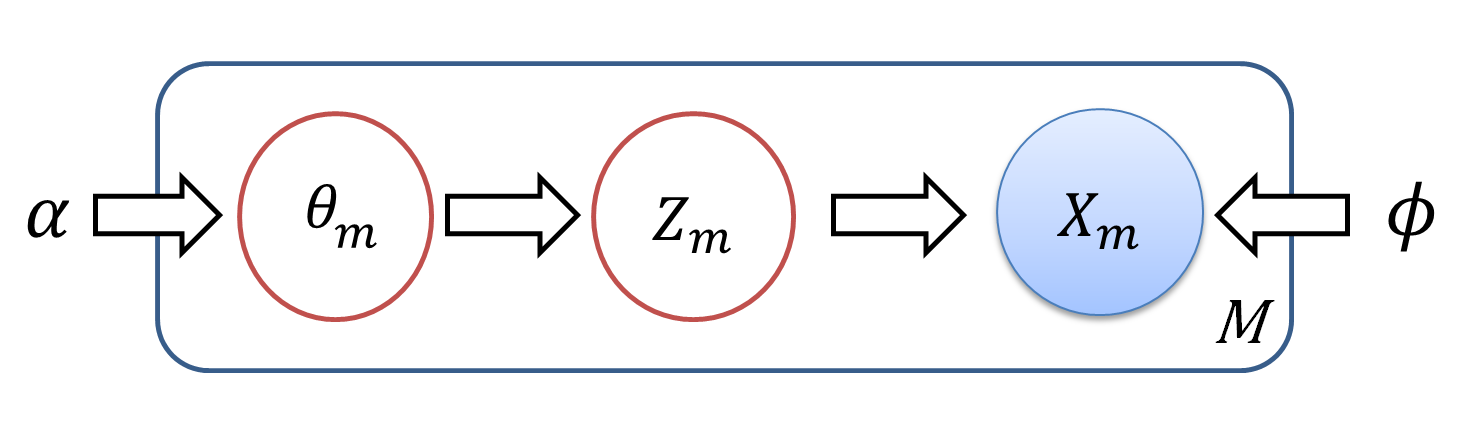
\includegraphics[width=0.9\linewidth, height=3.2cm,
        trim=0cm 0.5cm 1.2cm 0cm% height=1.2in0.75\textwidth% height=1.2in
        ]{FIGURES/LDA}
        \caption{Plate representation for LDA }
       % \vspace{-1.2cm}
    \end{subfigure}% ~   
    \caption{ Plate representation for  Gaussian Mixture Model (GMM) and Latent Dirichlet Allocation (LDA).
Shaded blue circles are observations, circles with red outlines are latent variables and symbols without circles are model parameters. %The blue rectangular plate represents  model is inferred at   particular structural level.
     }
     \label{Fig:GMMvsLDA} 
\end{figure*}

 

\subsection{ Mixture of Gaussian Mixtures (MGM)} 
 To overcome shortcomings of LDA, MGM is proposed by   Xiong et al. \cite{MGM} for distinguishing multiple types of group behaviours. % where MGM refers to Mixture of Gaussian Mixtures whilst for discrete features MGM is the Multinomial Genre Model.
  MGM is an adaptation of  Theme Topic Mixture Model  %proposed by  Keller  and Bengio 
  \cite{TTMM}  where instead of discrete datasets, MGM is constructed for continuous real-valued input data.  The MGM model introduces genres (themes) as mixtures of topics where each document is associated with certain genres.   %assumes% a group is a collection of documents where 
%  group memberships (collection of documents) are known a priori. 
  For example, books are naturally classified in terms of genres such as sci-fiction, romance, thriller and so on. Given a particular genre (type of regular behaviour), an anomalous group is characterised by an irregular mixture of topics.  %For $M$ groups, the $m$th group is specified by random vectors $ {\bf G}_{m}=\big\{ X_{mn}  \big\}_{n=1}^{N_m} $. 


In MGM, a document is  categorised by one of $J$ genres and a word in a document is generated from one of $K$ topics.   More specifically, the $m$th document is associated with latent variables such as genres $\chi_{m}$, genre mixtures $\theta_{m}$ and topics $Z_m$. 
The distributional parameters for topics, words and genres are respectively denoted with $\alpha,\phi,\gamma$.  
 The  posterior distribution in Equation  (\ref{pos})   for MGM is expressed as %   ${\bf X}= \{{\bf G}_{m},\dots,{\bf G}_{M} \} $ and model parameters are $\Theta=\{\alpha,\phi,\gamma\}$. 
 \begin{align*}
& \mbox{Observed Data:  \;\; \quad}  {\bf X}= \{{\bf G}_{1},{\bf G}_{2},\dots,{\bf G}_{M} \}\\
 & \mbox{Latent Variables: \quad}    \mathcal{H}=\{\chi_{m},\theta_m, Z_{m} \}_{m=1}^M  \\
 & \mbox{Model Parameters: \;\,}  \Theta=\{\alpha,\phi,\gamma\}
 \end{align*} 
  where ${\bf G}_{m} = \{ X_{mn} \}_{n=1}^{N_{m}}$ represents a group as a collection documents.  
  

We emphasise that in MGM, $  X_{mn} $ represents the $n$th document in the $m$th group rather than the LDA definition of the $n$th word in the $m$th document.   MGM is useful for modelling multiple groups of documents whereas a single document is a group of words for LDA.  
The MGM model also effectively learns multiple types of regular group behaviours however it may  fail to detect   point-based group anomalies  as it does not capture uncertainty of topic-word distributions. Without   Dirichlet prior distributions on topic-word probabilities in MGM, individual anomalies (specific anomalous documents) are poorly detected. 
 
 
 

\subsection{ Flexible Genre Model (FGM) }
 Xiong et al. \cite{FGM} extend MGM in a method called Flexible Genre Model (FGM).  Similar to MGM, multiple regular group behaviours are considered where a group or collection of documents is characterised by its topic  mixtures given a specific genre.  In addition, FGM  incorporates the uncertainties  of topic-word probabilities.   Dirichlet prior distributions in FGM account for  local document  structures as well as global group information  when estimating the topic-word probabilities.   This results in a better detection of point-based group anomalies as compared to MGM. 
 The topic-group weights are generated from a Dirichlet prior when data is discrete and Gaussian-Inverse-Wishart distributions for continuous real-valued datasets.
 
 Figure (\ref{Fig:FGM}) illustrates the graphical structure of FGM. MGM has a similar representation however it does not include Dirichlet priors on topic-word probabilities with $\phi_m \sim Dir(\beta)$. %With  additional Dirichlet priors,
  The posterior distribution for FGM is similar to MGM  except for additional latent variables  $\{ \phi_m\}_{m=1}^M$ and model parameters in FGM with $\Theta=\{\alpha,\beta,\gamma\}$ rather $\Theta=\{\alpha,\phi,\gamma\}$ in MGM. %For an appropriate comparison with MGM, FGM is also formulated for continuous real-valued data however it can also be adapted for discrete or categorical data.
     Overall, FGM is more effective than LDA and MGM for modelling multiple types of regular group behaviour as well as detecting point-based and distribution-based group anomalies. 

 
\begin{figure}[H]
\centering
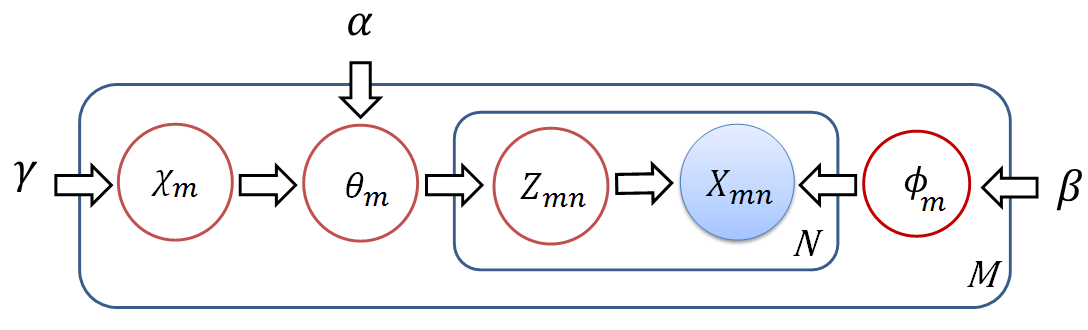
\includegraphics[width=14cm, height=4cm,trim=0cm 0cm 0cm 0.4cm]
{FIGURES/FGM} 
\caption{Graphical Representation of FGM where shaded blue circles contain observed data, unfilled  circles with red outlines are latent variables and symbols without circles are model parameters.}
%\vspace{-2cm}
\label{Fig:FGM}
\end{figure}
  

\section{Generative Models for Unknown Group Memberships}
We now elaborate on details of generative models where group memberships are unknown.   Clustering data instances into groups introduces an additional layer of  uncertainty and may not represent true group structures. Halkidi et al. \cite{ClusterValidity} discuss issues with the validity of clustering techniques %and F\~{a}rber et al. \cite{ClusterEval}  highlight that group labels may not even correspond to natural clustering structures.  
so a careful evaluation and interpretation of inferred clusters is required. % when true group memberships are unknown.
 To reduce the uncertainty of clustering data instances, Group Latent Anomaly Detection (GLAD) model \cite{GLAD} incorporates additional information from pairwise connections between data instances. %Yu et al. \cite{GLAD} find that the GLAD model has a relatively higher accuracy for inferring clusters given pointwise and pairwise data.
  Yu et al. \cite{GLAD} demonstrate the effectiveness of  GLAD in grouping data points compared to a number of graph-based clustering algorithms.



\subsection{ Group Latent Anomaly Detection (GLAD)} \label{subs:GLAD}
Detecting group anomalies becomes more challenging when memberships of groups are not previously known.  The  hierarchical structure  of GLAD utilises a combination of LDA as previously discussed and Mixed Membership Stochastic Blockmodel (MMSB) from Airoldi et al.  \cite{MMSB} to account for pairwise relationships between data points.  Similar to previous generative models, the $m$th group  is characterised by  topic proportions $\theta_{m}$ and an anomalous group is characterised by irregular topic proportions. % Yu et al. \cite{GLAD} demonstrate the effectiveness of  GLAD in clustering and  discovering group anomalies compared to a number of graph-based clustering algorithms.
A general drawback of the GLAD model is its input requirements of pairwise connection information that may not be readily available. 

The  graphical structure for the GLAD model illustrated in Figure \ref{Fig:GLAD} is noticeably different to FGM in Figure \ref{Fig:FGM}. Firstly without  prior distributions on topic-word probabilities $\phi_m$, GLAD may not be suitable for detecting point-based group anomalies. Also topic mixtures $\theta$ do not have prior distributions such that overfitting may occur if a large number of topics are examined. Compared to FGM and MGM, GLAD   does not account for multiple types of group behaviour. % Algorithm 3 further describes the  generative process of GLAD where
In Figure \ref{Fig:GLAD}, 
  ${\tilde G}_{n}$ represents a group membership indicator for the $n$th document with group membership  probability $\pi_n$. Topic variables $Z_n$ are inferred for each data point given their group membership.    The blockmodel parameter $\bf B$ contains  probabilities that documents in different groups share a connection. % one group has a connection with a document from another group. 
GLAD assumes discrete feature data  $ X_{n}$ and pairwise connections $Y_{n n'} \in \{0,1\}$  are respectively generated by  multinomial and Bernoulli distributions. Bernoulli probabilities represent the probability that there is a connection between the $n$th and $n'$th document. 

 The  posterior distribution %in Equation  (\ref{pos})   
$p({\bf X},\mathcal{H}| \boldsymbol\Theta) $ 
 for GLAD has %is summarised as %   ${\bf X}= \{{\bf G}_{m},\dots,{\bf G}_{M} \} $ and model parameters are $\Theta=\{\alpha,\phi,\gamma\}$. 
 \begin{align*}
& \mbox{Observed Data:  \;\; \quad}  {\bf X}= \{{\bf X}_{n} \}_{n=1}^N \mbox{ and } {\bf Y} =\{Y_{nn'}: 1 \le n,n' \le N \} \\
 & \mbox{Latent Variables: \quad}    \mathcal{H}=\{\pi_{n},\tilde{G}_n, Z_{n} \}_{n=1}^N  \\
 & \mbox{Model Parameters: \;\,}  \Theta=\{\eta,{\bf B},\theta, \phi\}
 \end{align*} 
  where the $n$th document is associated with one of $M$ groups with $\tilde{  G}_{n}  \in \{1,2,\dots,M\}$. 
  


 
\begin{figure}[H]
\centering
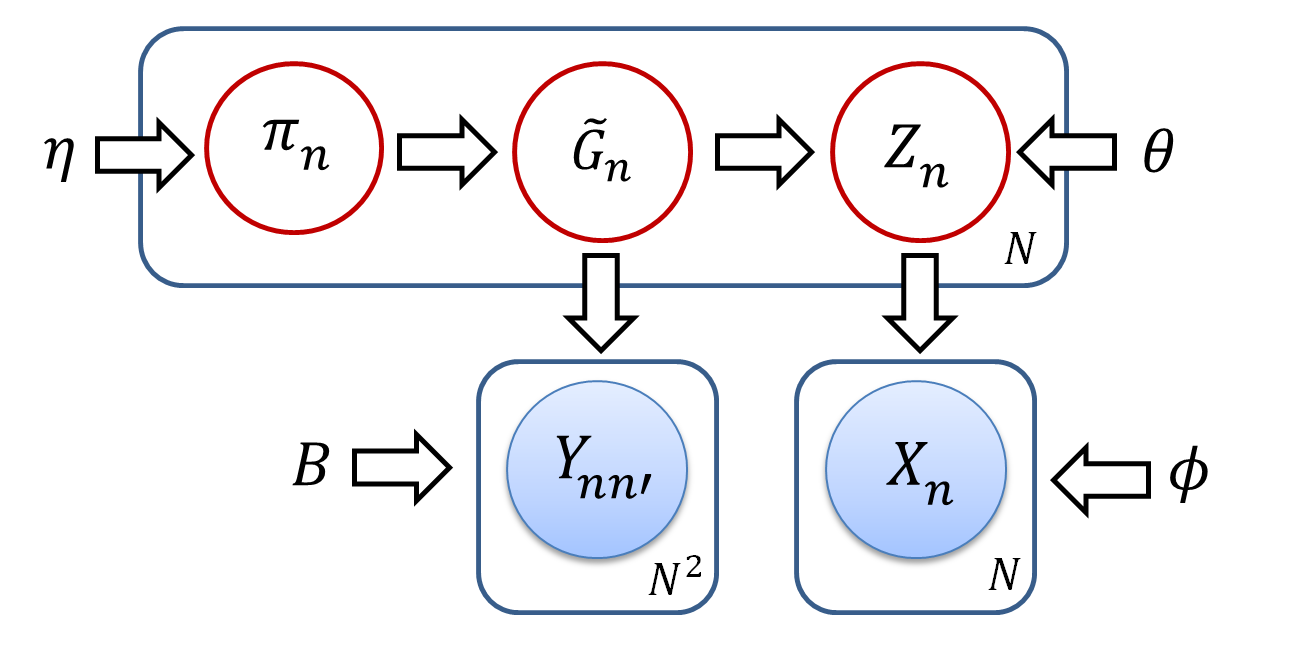
\includegraphics[width=12cm, height= 6cm,trim=0cm 0.6cm 2.5cm 0cm]
{FIGURES/GLAD} 
\caption{Graphical representation of GLAD where shaded blue circles represent observed data, circles with red outlines are latent variables and symbols without circles are model parameters.}
%\vspace{-2cm}
\label{Fig:GLAD}
\end{figure}


%\begin{landscape}
 \begin{table*}[H]
\begin{center}
 \scalebox{0.95}{
\begin{tabular}{ ccp{45mm}p{45mm}p{45mm}p{45mm}} 
 \hline\\%[-4mm]
Method & Data Variables $\bf X$ & Model Parameters $\Theta$ & Strengths & Weakness   \\%[1mm]
 \hline\\%[-4mm]
 LDA & $X_{m,n}$ &  $\alpha, \phi$ & Topic representation & Single topic mixture \\
 MGM & ${\bf G}_{m} $ %=\{X_{m,n} \}_{n} $
    & $\alpha, \phi,\chi$ & Multiple types of group behaviour & Cannot detect pointwise anomalies \\
  FGM & ${\bf G}_{m} $  & $\alpha, \beta,\chi$ & detect pointwise anomalies & Complex model \\
  ATD &  ${\bf X}_{m}  $   & $ beta, \phi$ & Incorporates sparse topic variables &  Requires labeled data \\
 %\multirow{2}{*}{GLAD} 
 GLAD & ${\bf X}_{m},{\bf Y}_{m} $   & $\alpha, beta, \psi, B$ & Simultaneously infers groups and detects anomalous groups &  Requires connection data \\
 %  OCSMM &  Group observations are IID  & Flexible representation of group behaviours. Does not require domain knowledge. & Choice of the kernel $k$. Sensitive to the parameter $\nu$ for the expected number of anomalous groups.\\
% KNNG-$\mathcal{D}$ &  Static & KNNG is nonparametric & No interpretation of anomalous group behaviour & \\ 
% MQCC & Dyanmic & Group observations are IID.
% Groups are independent over time. &  Requires training data\\
 %LRT & Dynamic & Group observations are IID.
% Groups are independent over time.  & & 
 \\ \hline
\end{tabular}
}
\end{center}
 \caption{Summary of Different Methods}
 \label{Tab:MH}
\end{table*}

%\end{landscape}


\section{Hypothesis Tests} 
\label{Sec:H}
 A hypothesis test is a specific type of generative model based on a null hypothesis or an assumption about how the data is generated. Instead of only computing a score such as in generative models, hypothesis tests also classify group deviations.  Hypothesis tests evaluate the statistical significance of an observed group with  a test statistic that captures the deviation of group observations from expected values. A statistical threshold is selected from the quantiles of a null distribution (assumed distribution following the null hypothesis).   The degree of anomalous behaviour in a group is quantified by a $p$-value or the likelihood that a group  observation is consistent with the null hypothesis. When multiple hypotheses are evaluated,  $p$-values require additional adjustment. 

 Many previous hypothesis tests have involved evaluating the equality of two groups in terms of different statistical properties. The equality of two groups has been evaluated using univariate means  in Student t-test,  multivariate mean vectors for Hotelling's $T^2$ test and univariate variances in  Barttlet's test.  There are also hypothesis tests involving more general properties such as empirical distributions in Kolmogorov-Smirnov test \cite{KStest}, multiple quantiles of two independent groups in Wilcox \cite{Wilcox1995} and quantiles of group difference distribution in Wilcox and Erceg-Hurn \cite{Wilcox2012}. The equality of multiple groups (greater than two groups) has also been studied for statistical properties such as multivariate mean vectors in MANOVA \cite{borgen1978uses},  count proportions in Chi-square test \cite{kass1980exploratory}  and covariance matrices in Box's test \cite{box1954some}. The above hypothesis tests are more effective for testing the equality of groups  however  do not explicitly classify anomalous  group behaviours. % but rather determine if there is a difference in group behaviours. 
 
 
%\begin{center}
%{\bf Advantages and disadvantages of  hypothesis testing}\\ 
%Advantages:
%\begin{enumerate}[(1)]   \setlength\itemsep{5pt}
%\item Flexible formulation  of how data is generated 
%\item Offers clear interpretation of results 
%%\item  Directly classifies group behaviours as regular or anomalous
%\item Quantifies the statistical significance of a group   
%%\item    Can be applied in a supervised or unsupervised manner % group anomaly detection
%\end{enumerate} 
%Disadvantages:
%\begin{enumerate}[(1)]   \setlength\itemsep{5pt}
%\item    Assume data follows a particular distribution under the null hypothesis 
%%\item  Results are sensitive to initial parameter  selection  
%\item Prone to overfitting for multiple hypotheses
%\end{enumerate} 
%\end{center}

 
\subsection{Anomalous Topic Detection (ATD)} \label{Sec:ATD}
In the context of topic modelling,  Soleimani \& Miller \cite{ATD} introduce  Anomalous Topic Discovery (ATD), a supervised learning approach that clusters anomalous
documents when memberships are previously unknown. The regular behaviours of documents are extracted from an appropriate training set with discrete data inputs. ATD implements a non-parametric bootstrap sampling procedure to  evaluate the statistical significance of a detected anomalous behaviour for a single document as well as a cluster of documents.     
Like in previous analysis, groups are  characterised by topic variables however an anomalous group is not characterised by irregular topic proportions. Instead  a group anomaly in ATD  is defined as a cluster with an additional topic that is not explained by  regular topics inferred from a training set.   


ATD learns topics using  Parsimonious Topic Model (PTM) proposed by Soleimani \& Miller  \cite{PTM}. % as PTM has many advantages over the simpler LDA model. 
%From Soleimani \& Miller  \cite{PTM}, 
PTM is more effective than the simpler LDA model for handling sparse topic representations in high-dimensional datasets by  incorporating  globally shared topics as well as topic-specific variables.   
  Rather than estimating  parameters through  Monte Carlo simulations or variational inference,  PTM  reduces computational burden by selecting models based on comparing information criteria.     
After clustering documents based on  topics  inferred from PTM, the ATD method evaluates the statistical significance of an anomalous cluster using a non-parametric bootstrap approach.  Figure \ref{Fig:ATD} summarises the clustering process and significance testing of anomalous documents in ATD.  %It is possible to apply other generative models such as LDA or MGM in the ATD method in order to classify groups with statistical significance rather than calculate group deviation scores. 
 
If we assume $K$ regular topics are inferred from a training set then ATD evaluates a cluster $\mathcal{C}$ based on the following hypothesis :
\begin{align}
&\mbox{ $H_0:$ Cluster $\mathcal{C}$ has $K$  regular topics } %\nonumber \\
 \mbox{ \, versus \, $H_1:$ Cluster $\mathcal{C}$ contains  $K+1$ topics }
\label{Hyp:ATD} 
\end{align}
where an additional topic is seen as anomalous. 

We explain details of ATD using the four key components from Section \ref{Sec:Problem}. 
\begin{enumerate}[1.]
\item Characterisation function $f_1({\bf G}_{train})=l_0(\mathcal{C})$: \\ 
ATD estimates $K$ regular topics and other  parameters  of a null model under $H_0$  from  training set ${\bf G}_{train}$.  
 %A hypothesis test in ATD evaluates whether  is appropriate for a test cluster. 
%This null model characterises the training set by  $K$ regular topics. 
The probability that a cluster $\mathcal{C}$ is generated under null hypothesis $H_0$  is denoted by 
$l_0(\mathcal{C}) = \sum_{n  \in \mathcal{C} } \ln p( n| H_0 ) $. 
\end{enumerate}
%
\begin{enumerate}[2.]
\item Characterisation function $f_2({\bf G}_{test})=l_1(\mathcal{C})$: \\
%We do not fully elaborate on the details of PTM, but rather focus on the ATD method. 
  Figure \ref{Fig:ATD} illustrates the process of inferring a significantly anomalous cluster with the maximum deviance  from the null hypothesis $H_0$.  
%   the ATD method for aggregating data instances into a test cluster and evaluating the presence of additional anomalous topics. % ATD is a supervised method where  regular  topics is inferred from a training set. 
 Anomalous documents from a test set  are  iteratively added to a test cluster $\mathcal{C}$ until  no  statistically significant anomalous topics are detected.   %A test cluster is then evaluated for $|\mathcal{C}|>4$.
  A test set ${\bf G}_{test}=\mathcal{D}'$ is updated by omitting the anomalous cluster where $\mathcal{C}$ is characterised by $K+1$ possible topics under hypothesis $H_1$. The likelihood  that a test cluster contains an additional topic is $l_1(\mathcal{C}) = \sum_{n \in \mathcal{C} } \ln p(n | H_1 )$. 
 %Documents with significantly anomalous behaviours are added to a test cluster in an iterative process.  
%   A test cluster  $\mathcal{C}$ requires at least 4 documents () before evaluating its anomalous behaviour.  %Similar to previous generative models, a test cluster  is a collection of documents where each document is characterised by topics. %  Since an anomalous cluster is previous unknown, naive search would take $2^{|\mathcal{D}^t|}$ subsets of a test set. 

% ATD finds a cluster $\mathcal{C}$ with  maximum deviance from the null hypothesis by the iterative process portrayed in Figure \ref{Fig:ATD}. 
%This likelihood is treated as an anomalous score. 
\begin{figure}[h]
\centering
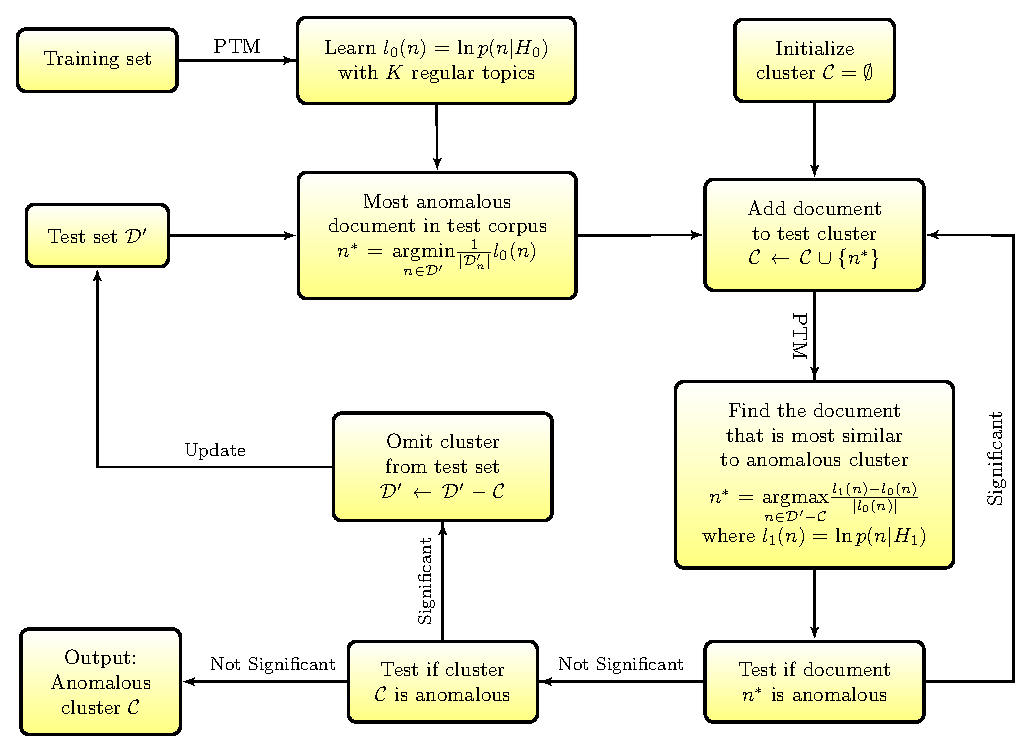
\includegraphics[width=14cm, height=10cm, trim=0cm 0cm 0cm 0cm]
{FIGURES/ATDfigure} 
\caption{ Illustration of the clustering procedure using Anomalous Topic Discovery (ATD)  }
%\vspace{-2cm}
\label{Fig:ATD}
\end{figure}

\end{enumerate}
%
\begin{enumerate}[3.] 
\item Measure $ \mathcal{D}\big(f_1 ({\bf G}_{train}) , f_2({\bf G}_{test} )\big )= l_1(\mathcal{C})  -l_0(\mathcal{C})$: \\
An anomalous score for a test cluster $\mathcal{C}$ is computed by the log-likelihood ratio  
\[\mathcal{S}(\mathcal{C})= l_1(\mathcal{C})  -l_0(\mathcal{C}) =   \sum_{n  \in \mathcal{C} } \ln \frac{p( n| H_1 )} {p( n| H_0 )} \]
which quantifies the probability that a cluster contains a significantly different topic from $K$ regular topics inferred from  training data. Other generative models only calculate group deviation scores however ATD also evaluates the statistical significance of a test cluster. 
% An anomalous measure  is calculated by a $p$-value or likelihood that a test cluster is consistent with the null hypothesis. A parametric distribution for group deviation scores is not assumed as clusters may have small sample sizes. % as $|\mathcal{C}|>4$. 
  A non-parametric bootstrap procedure is  applied  where the null distribution is estimated by sampling documents from the  training set.  Scores for $B$ bootstrap clusters are respectively denoted by    $\mathcal{S}(\mathcal{C}_1),\mathcal{S}(\mathcal{C}_2),\dots,\mathcal{S}(\mathcal{C}_B)$ and an empirical $p$-value for test cluster scores is calculated by    
\[ \frac{1} {B+1} \sum_{b=1}^B \Big[I \Big(b : \mathcal{S}(\mathcal{C}_b) > \mathcal{S}(\mathcal{C}) \Big)+1 \Big] \]
where $B$ is the number of bootstrap simulations. 
  Further details of bootstrapping procedures for ATD are described in Soleimani \& Miller \cite{ATD}. 
\end{enumerate}
\begin{enumerate}[4.]
\item Threshold $\epsilon=\alpha$: \\ 
Once a $p$-value is calculated, a statistical threshold is selected from the quantiles of the null distribution generated from bootstrap simulations. 
Soleimani \& Miller \cite{ATD} do not describe multiple hypothesis testing issues for iteratively evaluating   anomalous documents or test clusters. Thus a  test cluster is considered anomalous if the empirical $p$-value is less than a pre-selected  significance level $\alpha$. 
\end{enumerate}
 
 
\subsection{Extreme Rank Anomalous Collection Detection (ERACD)}
Dai et al. \cite{ERACD} introduce Extreme Rank Anomalous Collection Detection (ERACD), an unsupervised approach that evaluates the statistical significance of  inferred clusters % collections of data instances 
 where group memberships are previously unknown. ERACD aggregates data instances into anomalous clusters based on extreme rankings. Group anomalies are characterised by a variety of extreme features such that multiple hypotheses evaluate the significance of group deviations. % and evaluated using a Bonferroni correction method \cite{Bonferroni}. 
The ERACD  algorithm detects both a point-based group anomaly as a large number of entities with a single extremely ranked feature or a distribution-based group deviation where entities have extreme ranks across multiple features.

ERACD has many advantages over other state-of-the-art methods. 
The ERACD  algorithm focuses on a relatively small number of members in clusters whereas many other methods require larger group sizes. Dai et al. \cite{ERACD} find that ERACD infers clusters with more anomalous behaviours compared to other clustering techniques.  Hypothesis tests in ERACD also provide an explanation for the deviating statistical properties of a group anomaly. % based different assumptions of independent and dependent feature sets.  
ERACD requires model parameters such as the number of expected anomalous clusters and the maximum allowable size for clusters.  % Model selection in ERACD is difficult  to automate and evaluate without sufficient labeled data. 
  The effectiveness and interpretation of results is sensitive to initial parameter selection.   
 %Due to the flexible framework of ERACD, it can be applied to networks data where feature data for a particular node is obtained by the path distance to different entities in a cluster. 

  Since the detection of distribution-based anomalous clusters across multiple features requires more elaborate details, we describe key components of ERACD for detecting point-based group anomalies as follows.  
A general hypothesis involving the $v$th feature of a test cluster $\mathcal{C}$ can be stated as 
\begin{align}
&  \mbox{ $H_0:$  $v$th feature of cluster $\mathcal{C}$ is regular}  \mbox{ \, versus \, $H_1:$  $v$th feature of cluster $\mathcal{C}$ is anomalous   }
\label{Hyp:ERACD} 
\end{align}
where multiple hypotheses are evaluated over different  statistical properties with features $v=1,\dots, V$.  

\begin{enumerate}[1.]
\item Characterisation function $f_1({\bf G}_{train})=|{\bf X}_{v} (r)|$: \\ 
%The entities that contains extreme features is  an extremity index $r$ 
Consider $N$ data instances each with $V$ features where the rank of feature $v$ for the $n$th data instance is denoted by $rank_v(n)$ for $n=1,2,\dots,N$. 
Based on the $v$th feature, data instances in the training set
 $\bf X$ with  top $r$ rank positions (highest values) are examined according to  
\begin{align}
{\bf X}_{v} (r) = \{n |n \in  {\bf X}, \, rank_v(n) \le r \} \label{Eqn:Rank}
\end{align} 
ERACD characterises the training set by the number of elements  with $|{\bf X}_{v} (r)|$. 
%Since ties may occur in a dataset, it is possible that the $n$th and $n'$th instance have $rank_v(n)=rank_v(n')$. Generally
with  the $r$th rank  of feature $v$ satisfying   $ | {\bf X }_{v} (r) | \le r$. 
 %Rather than examining regular behaviours in training data,
 The function $f_1$ characterises regular behaviour of a training data for  extreme ranks of features.   

\end{enumerate}

\begin{enumerate}[2.]
\item Characterisation function $f_2({\bf G}_{test}) = |{C}_{v} (r)|$: \\ 
ERACD  algorithm infers group structures using an iterative pruning technique based on anomaly scores.  The  top $r$ rank positions of the $v$th feature for cluster $\mathcal{C}$  is given by 
\begin{align}
{C}_{v} (r) = \{n |n \in \mathcal{C}, \, rank_v(n) \le r \} \label{Eqn:Rank}
\end{align} 
Similarly, ERACD characterises a test set by the number of elements in a test cluster   with $|\mathcal{C}_{v} (r)|$. 
%By only examining a single feature, point-based group anomalies are detected however distribution-based anomalous clusters are discovered based on extreme ranks across multiple features.  
\end{enumerate}


\begin{enumerate}[3.] 
\item Measure $ \mathcal{D}\big(f_1 ({\bf G}_{train}) , f_2({\bf G}_{test} )\big ) = {p}_v(\mathcal{C},r^*)$: \\
Cluster ${C}_{v} (r)$ is compared with $ { \bf X}_{v} (r) $ to  identify point-based anomalous clusters for the $v$th feature. 
%To test if an inferred cluster is anomalous with respect to its $v$th feature,
 The null hypotheses in ERACD assumes that  randomly selecting  entities (with top ranked features)  in a collection $\mathcal{C}$ as compared to the whole dataset $\bf X$ follows a  hypergeometric distribution. 
A hypergeometric probability with parameters $a,b,c,d $ is given by
\begin{align}
 P(a,b,c,d) = \displaystyle \frac{ {a+b \choose{a} } { c+d \choose{c} } } { {N' \choose{a+c} } } \label{Eqn:hyperG}
\end{align} 
where the total count is $N' = a+b+c+d$. 
  If a group is characterised by top $r$ ranks of feature $v$, a $p$-value is calculated from the upper tail with  
 \[           p_v( \mathcal{C} ,r ) =  
 \displaystyle \sum_{n = |\mathcal{C}_v (r) | |} ^ {\min(| {\bf X}_v (r) |,| \mathcal{C}| )}  P (n, N,|{\bf X}_{v}  (r)|,|\mathcal{C}| ) \]
where probabilities are given by the hypergeometric distribution  in Equation (\ref{Eqn:hyperG}). In practice, the selection of parameter $r$ is difficult and Dai et al. \cite{ERACD}  define a representative value with   
%\begin{align}
$r^* = \underset { 0 < r < N/2 } { \mbox{argmin}} \,  p_v( \mathcal{C} ,r )$ % \label{Eqn:RepInd}
%\end{align}
For a particular feature,  a representative $p$-value $p_v( \mathcal{C} ,r^* )$  is a more appropriate measure for  extremely ranked behaviour of a cluster, compared to using $p$-values with a different value of $r$. %entities with extreme ranks from training data.  
   
\end{enumerate}
\begin{enumerate}[4.]
\item Threshold $\epsilon=\alpha/V$: \\ If a single hypothesis is evaluated for an inferred cluster  then a $p$-value is significant if it is less than  a pre-defined significance level  $\alpha$. Since ERACD evaluates $V$ hypothesis to search for features that characterise anomalous clusters,  a Bonferroni adjustment \cite{Bonferroni}  is applied where a test cluster  is anomalous if % it has a $p$-value less than the following threshold
\[  {p}_v(\mathcal{C},r^*) < \alpha/V \]   
\end{enumerate}

